\chapter{Expanding to the CCUC-problem}\label{CCUC}
With the CCRC-problem solved it is time to move towards a problem that lies within the realm of reality, the CCUC-problem.
For the CCRC-problem the reality of wireless technology was warped with the assumption that communication is perfect.
For the CCUC-problem this assumption amongst a few others will be removed; as such certain aspects of the CCRC-solution will be adapted to fit the CCUC-problem.

This adaptation to the CCRC-solution must consider not just the chance for packet loss to occur, but also the effect.
As going from reliable to unreliable communication is the only change that occurs some parts stay the same; the rest of this chapter will focus on the aspects of the CCRC-solution which do change.

%Frame intact
%How to sufficiently guarantee communication, what is sufficient?
%WorstCase different
%Time-Slots guard time/padding required
%Consensus in network for certain actions

\section{Package Loss}
As we are now working with a realistic scenario of unreliable communication one must also realise that this is an impossible problem to solve completely.
As one can never guarantee that a packet will be received, the best one can do is reduce the odds of it happening.
Adjusting the UPPAAL model in, \myref[name]{sec:uppaalccuc}, to account for a 2~\% packet loss, which is more than the results in \myref{tbl:packageloss} show, the network works approximately 96~\% of the time.
As mentioned one cannot reach 100~\% when considering unreliable communication, however this does not mean that nothing can be done.
By employing different methods to increase the odds of packets being received one can attempt to approximate a reliability of \textasciitilde100~\%.

Another aspect of unreliable communication is the effect of packet loss.
Depending on what data is being transferred the impact of packet loss differs.
In regards to small data packages such as those this protocol uses for network management, packet loss completely corrupts the payload.
As such aside from implementing methods to decrease the odds of packet loss, one must also consider what the repercussions of packet loss will bring and if possible reduce this as much as possible. 

\subsection{Methods of Avoidance}\label{sub:avoidance}
As aforementioned one can attempt to approximate 100~\% reliability in a network by reducing the odds of package loss.
In an effort to reduce package loss two ideas will be presented, both based on the concept of conditional probability, a subject of probability theory.

\subsubsection*{Message Redundancy}\label{redundancy}
If a time-slot was extended such that a device has time to transmit the same payload more than once, then the probability of the other devices not receiving the transmission will be reduced, and thus increase the reliability of the network.
While the increase in probability the time-slot length will be increased, and thus the network will become slower.
Therefore this is a trade-off between time and reliability. 

\subsubsection*{Multimessage Echo}
It could be useful to repeat the last $x$ received messages a device have heard in its own time-slot, such that if other devices had not heard a messages, they could be heard from this.
This would echo messages from devices several times over, but from different devices which in the case that the problem is between two devices could help where Message Redundancy might not.  
Furthermore this would implicitly allow for devices to hear whether or not another device heard them, given their time-slots are within the amounts of messages echoed.
Moreover echoing can increase the message length greatly, and thus will also reduce the speed of the network as message redundancy would.
The size of this reduction would be dependant on how many messages are being echoed. 
\subsection{Package Loss and Damage Control}
As one cannot reach complete reliability one must consider the effect of a packet being lost regardless of how low that chance may be.
While the effect of packet loss is different depending on what data is being transfered, for the protocol in this paper corrupt data will render the transmission useless.
On the off-chance that a device completely misses a package regardless of any avoidance methods used, it should be able to recover and continue in the network without issues; furthermore in the case that the data was of importance to the device which missed it, this information should somehow be relayed back to the device that transmitted the message.
This way the previous data can be retransmitted if it was of any importance to the device which missed it.
Another problem faced is that syncing is handled through received transmissions, as such missing a transmission could cause desynchronization, however this would only occur with either a significant clock drift, or a significant amount of continuous transmissions missed as the time-slots are fixed.
The following two methods could help in the case of packet loss.

\subsubsection*{Continuous listening}\label{contListen}
This idea is presented in order to resolve the larger part of the issue, potential desynchronization.
Should a package be missed, a device will simply begin listening until either it receives a new transmission, or the device should transmit.
As a transmission is received the procedure \texttt{protocolMaintaince}, \myref{lst:maintaniance}, is not run and as such it is possible that the device may be slightly out of sync.
Listening until a new transmission is received allows the device to sync up with the rest of the network and as no transmission was received, there is no reason to run usercode.
In the case where no transmission is received prior to a devices time-slot, it will still transmit.
This is necessary as otherwise a dead device would effectively put the network in an eternal state of listening.
As mentioned however the device might be slightly out of sync, for this reason it makes sense to add guard time for padding; this would ensure that devices start listening prior to a given device transmitting even if they are completely sync.
Effectively this is already part of the protocol as the first part of $\delta_{comm}$ is to make a payload which as it happens provides enough padding to resolve the desynchronization due to it being so slight.

\subsubsection*{Bitfield Time-Slot ID Index}
The idea presented in this section allows devices to know whether or not they have been heard.
As part of any device's payload one could add a bitfield where each bit denotes a device in the network.
As all time-slots have their own ID and and each device know the active time-slot, they can transmit a bitfield representing whether or not they heard anything in time-slot 1 to n.
This would allow devices a memory and time efficient way of delayed acknowledgments.
This, to a degree, resolves the issue of a device not received a payload which was of some importance to that device.
The reason why this is not completely solved is that the original device which sent the first payload, could in theory miss the payload from the device for which the payload was intended, as such the first device would not know the intended device had not received the payload.
This however is part of the reason why one cannot achieve 100 \% reliability.

\section{Cause and Effect}
Due to the unrealiability of communication some previously designed parts of the protocol should be changed in order for the protocol to work more reliably, these areas are described in this section.
\subsection{Frame and Time-Slots}

GuardTime

TimeSlotLength
\subsection{Worst Case}
WorstCase can no longer be determined
Due to the new stochastic design
\subsection{Consensus}
Each device stores certain local variables which preferably should be consistent across devices by the end of a time-slot.
If this is not the case, it is the result of one or more devices either not knowing that a new device has joined, or that one has been removed.

These variables should essentially be globally available but as this is not possible, they are stored as local variables and transmitted in each payload.
With the CCRC-problem one could blindly trust that all information which had been transmitted would also be received which is not the case with the CCUC-problem.

\bigskip \noindent
For this reason the idea of a consensus between devices is presented, to explain this imagine the scenario where a device is attempting to join the network.
After having been validated, the device will in the empty slot join the network with a different $n$ and a different $k$ relative to the devices in the network.
In the earlier CCRC solution one would simply overwrite local variables with the new values as one was sure all had received the payload.
In the case where one device did not hear the addition, it would be transmitting the old variables and in doing so cause the change to revert back again, which by extension causes a conflict in the network.
It is worth mentioning this is only a problem if it possible for n to be reduced, i.e. the removal of devices is possible.
If the removal of a device from a time-slot is not enabled, anytime an $n$ larger than the local $n$ is being transmitted, this should just overwrite the local value. 
However as soon as removal is also an option, a device cannot just trust any n-value as variables can both increase and decrease, and a device transmitting a lower value, might just do to because it does not know about the new device yet.

If one instead establishes a consensus by listening to the majority of the network; one device will no longer be able to create a conflict.
The majority would have to be determined by the following frame as all removals and additions to the network are handled in the second to last and last time-slot respectively.
Furthermore one could introduce a mode which denotes that a device wants to either increment or decrement $n$, once the device that initiated the change has received a payload with a response to the request from all other devices, $n$ should be changed for the entire network, and devices will then accept any change according to the request from any device.
The request it will keep being transmitted until all devices respond that they are ready to act upon it by either incrementing or decrementing their $n$ value.
Furthermore whilst this request is being transmitted, no new device should be able to join the network, and the other devices in the network should also transmit the request, to increase the speed of which it will be spread throughout the network.
\subsection{Payload}
Dmg control and consensus

\section{Adaptation of CCRC-Solution} % (fold)
\label{sec:adaptation_of_ccrc_solution}
Due to time constraints in regards to this project, the first order of business in the adaptation of the CCRC-solution to the CCUC-problem, is to choose a subset of the ideas presented in the previous sections.
This limitation is also imposed to ensure a more ``depth first'' approach where the selected ideas are throughly designed, validated and implemented.

As a consequence of that decision, the idea of message redundancy as presented in \myref[name]{sub:avoidance} will be subject to further design and validation during the CCUC-problem.

In order for the message redundancy to be introduced into the existing solution from the CCRC-problem, only minuscule changes must be applied.
\begin{enumberate}
    \item The transmission phase which takes $\delta_{comm}$, must be expanded to account for more transmissions of the same length; and
    \item the receiving phase must likewise be expanded.
\end{enumberate}
These relatively small changes must be validated and the increase in reliability, if any, will be presented.
However firstly the UPPAAL-model from \myref[name]{sec:themodel} must be adapted to express the CCUC-problem, i.e. the chance of missing a transmission from another device.

% section adaptation_of_ccrc_solution (end)

\section{Model Checking the CCUCprotocol}
This section will utilise UPPAAL to see what happens with the model when unreliability is introduced to the model.

The changes to the model are that whenever something is received, it will have a chance to miss the transmission, and therefore not fire the edge which receives the transmission.
This can be modelled in UPPAAL using the branch points as seen on \myref{fig:missTransmission}.

\begin{wrapfigure}{R}{0.3\textwidth}
\centering
  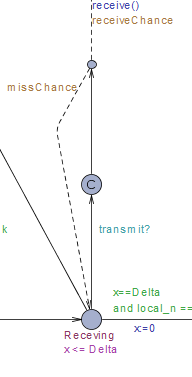
\includegraphics[width=0.3\textwidth]{Figures/Model/MissChance.png} 
\caption{Graph showing the split node after receiving, where there is a chance for the device to miss the transmission and go back to the same location.}
\label{fig:missTransmission}
\end{wrapfigure}

The chances \texttt{missChance} and \texttt{receiveChance} are simply created so the sum of them is 100 and this is shown in 

\begin{lstlisting}[style=UPPAAL, title={The creation of }]
4. Pr[<=300000] Pr[<=300000] ( <>  forall(i : id_t) (time >3000) 
    and Device(i).local_n == N + 1)
\end{lstlisting}

